%!TEX TS-program = pdflatex
%!TEX encoding = UTF-8 Unicode
\documentclass[11pt,a4paper,english]{article}

\usepackage[utf8]{inputenc} %input chars
\usepackage[english]{babel} %language
\usepackage[T1]{fontenc} %output chars
\usepackage{lmodern} %font
\usepackage{geometry} %page layout
\usepackage{amsfonts} %math symbols
\usepackage{amsmath} %math equations
\usepackage{amssymb} %math symbols
\usepackage{mathtools} %other math
\usepackage[numbers]{natbib} %bibliography
\usepackage[nottoc]{tocbibind} %other bib
\usepackage{paralist} %lists
\usepackage{graphicx}
\usepackage{subcaption}
\usepackage{multirow}
\usepackage{multicol}
\usepackage{pgfplots} %plots
\usepackage{listings} %listings
\usepackage{epstopdf} %eps images
\usepackage{color} %colored text
\usepackage{algorithm2e}
\usepackage{float} %images going to end of the document
\usepackage{hyperref}
\makeatletter
\newcommand{\HEADER}[1]{\ALC@it\underline{\textsc{#1}}\begin{ALC@g}}
	\newcommand{\ENDHEADER}{\end{ALC@g}}
\makeatother
\usepackage{microtype} %better type
% questo sono i default per i listings 
\lstset{
	frame=tb, % draw a frame at the top and bottom of the code block
	tabsize=4, % tab space width
	showstringspaces=false, % don't mark spaces in strings
	breaklines=true,
	numbers=left, % display line numbers on the left
	basicstyle=\footnotesize,
	commentstyle=\color{green}, % comment color
	keywordstyle=\color{blue}, % keyword color
	stringstyle=\color{red} % string color
}

\DeclareRobustCommand{\univsc}[1]{\Large\textsc{\textls[75]{#1}}}
\DeclareRobustCommand{\titlesc}[1]{\linespread{1.2}\LARGE{\textls[35]{\uppercase{#1}}\linespread{1}}}
\DeclareRobustCommand{\namesc}[1]{\large\textsc{\textls[35]{#1}}} 

\newcommand{\facciatabianca}{\newpage\shipout\null}

\allowdisplaybreaks

\begin{document}
	
\pagenumbering{Alph}
\begin{titlepage}
	
	\begin{center}
		%	\includegraphics[width=2cm]{logo_univ_udine}
		\vbox to0pt{\vbox to\textheight{\vfil
{\tiny }				
\includegraphics[width=0.93\textwidth]{polloPallido}\vfil}\vss}
	\end{center}
	
	\begin{center}  
		\univsc{Scuola Superiore\\dell'Universit\`a degli Studi di Udine}
		\medskip   
		\rule{10cm}{.4pt}\\
		\medskip\begin{Large}
			{Classe Scientifico-Economica}\\    % Eventualmente Classe Umanistica
			\medskip
			\vspace{\stretch{0.6}}
			Colloquio di fine anno\end{Large}\\
		\medskip
		\vspace{\stretch{0.25}}
		\titlesc{Tensorflow probability - Probabilistic programming with Tensorflow and physical applications}       % Inserire il titolo
		
		\bigskip\vfill
		\large
		\begin{tabular*}{\textwidth}{@{}l@{\extracolsep{\fill}}r@{}}
			\large Relatore:&Allievo:\\			% Eventualmente cambiare Allievo con Allieva. 
			% Relatore va lasciato invariato anche se è una donna.
			%  
			%Se il titolo onorifico del relatore è troppo lungo per stare sulla stessa riga (es:Chiar.mo Prof.)
			%cancellare il simbolo % nella riga qui sotto, sostituire i dati e inserire % all'inizio delle 2 righe sotto
			%Chiar.mo Prof.& \namesc{Nome studente}\\\namesc{Nome docente}&
			Prof.
			\namesc{Scagnetto Ivan}&% Inserire il nome del relatore. 
			% Se il relatore è un ricercatore sostituire Prof.\ con Dott.\
			% Se il relatore è una donna sostituire con Prof.ssa o Dott.ssa  															
			\namesc{Corrado Alessio}				% Inserire il proprio nome
			
		\end{tabular*}
		
	\end{center}
	
	\begin{center}
		\vfill
		\rule{10cm}{.4pt}\\
		\medskip
		\univsc{Anno Accademico 2019-20}\\  %verificare che l'anno accademico sia quello 
		%in cui si è seguito il corso su cui si è svolta la tesina 
	\end{center}	
	
\end{titlepage}
%\clearpage{\pagestyle{empty}\cleardoublepage} 
% In caso di inserimento nel file della tesina, 
% il comando produce una pagina bianca dopo il frontespizio. 
% Rimuovere se in caso di stampa solo fronte.

%se non funziona usare questo che è brutale
%\newpage\shipout\null\stepcounter{page}

\newpage

\tableofcontents

\newpage
\pagenumbering{arabic}

\section{Introduzione} 

\paragraph{} Lo scopo del progetto è la realizzazione di un \textbf{file storage distribuito}\cite{distributedfs}. 

\paragraph{} Le caratteristiche che deve avere sono:

\begin{itemize}
	\item \emph{Efficienza}: I tempi di risposta devono essere ragionevoli e non degradare con l'aumento del numero di nodi. L'utilizzo delle risorse a disposizione deve essere massimizzato, ovvero non devono esserci risorse inutilizzate o carichi di lavoro troppo sbilanciati.  
	
	\item \emph{Accesso concorrente}: Più client possono effettuare richieste in modo concorrente. Deve essere tenuta in considerazione qualche politica di \emph{fairness}, 
	in modo che nessun client sia eccessivamente privilegiato o venga escluso. Deve essere garantita la \emph{consistenza} specificamente in caso di accessi concorrenti alla stessa risorsa. 
	 
	\item \emph{Replicazione dei dati (files)}: Per garantire un buon livello di \emph{fault tolerance}, tutti i dati devono poter essere replicati. In questo modo problematiche su un nodo non compromettono il contenuto di un file. 
	
	\item \emph{Replicazione dei metadati (struttura del fs)}: La struttura del \emph{file system} deve essere sempre replicata, in modo che non possa essere persa o corrotta .
	
	\item \emph{Disponibilità e consistenza}: deve essere massimizzata la disponibilità delle risorse, mantenendo al contempo una consistenza forte. In particolare, ogni richiesta deve riferirsi all'ultima versione della risorsa (se non diversamente indicato).  
	
	\item \emph{Sicurezza}: Deve essere curata la gestione della sicurezza: sia a livello di connessione (utilizzando opportunamente cifratura e autenticazione) che di accesso (autenticazione dell'utente, privilegi sul fs). Deve essere minimizzata l'esposizione ad attacchi malevoli. Deve essere possibile ripristinare il sistema a seguito di un attacco o errore. 
\end{itemize} 



\paragraph{Numero di repliche dei dati}

Il numero di repliche di un file deve essere \underline{proporzionale} sia all'importanza che al numero di accessi di esso: documenti con \emph{dati critici} hanno numero di copie maggiore, per agevolarne la \emph{disponibilità} e diminuire le \emph{probabilità di perdita}. 


\paragraph{Bilanciamento del carico} Per migliorare l'efficienza viene effettuato un bilanciamento del carico: in ogni momento il sistema può \underline{copiare} o \underline{spostare} dati in modo da non sovraccaricare un singolo nodo. Inoltre, per il trasferimento in uscita di un documento si cerca di utilizzare il nodo con maggiore \emph{banda disponibile}. 



\section{Architettura del sistema}

Verranno di seguito analizzate diverse possibili architetture del sistema, comparandone pregi e difetti. 

\subsection{Single-server}

\paragraph{} La prima idea è quella di avere un \emph{singolo server}, il quale memorizza \emph{sia la struttura del fs che i dati}. Il client interagisce direttamente con esso per effettuare qualsiasi operazione. 

\paragraph{} Il fs può essere memorizzato a partire da una \emph{directory nel filesystem del server}, oppure in una \emph{partizione separata}. Con entrambe le soluzioni è il sistema operativo ad occuparsi della sua gestione.

\paragraph{} La \emph{replicazione dei dati} avviene mediante il salvataggio in \underline{diversi dispositivi di memorizzazione} (es HDD). Per far ciò la scelta più consona è di utilizzare un sistema \textbf{RAID 10}\cite{raid}: i dati vengono \underline{salvati in copia} (RAID 1) per avere \emph{tolleranza ai guasti} e in \underline{striping} (RAID 0) per aumentare la \emph{velocità di lettura}. 

\paragraph{} Con \underline{schede di rete (e connessioni) multiple} è possibile migliorare la tolleranza sia ai \emph{guasti} che alle \emph{congestioni di rete}. 

\paragraph{Vantaggi} \begin{itemize}
	\item Semplice da implementare.
	\item Modello più economico.
	\item Il fs è gestito direttamente dal sistema operativo.
	\item Minima esposizione contro attacchi hacker.
	\item Con gli accorgimenti sopra descritti si ha già una buona fault tolerance. 
\end{itemize} 

\paragraph{Svantaggi} \begin{itemize}
	\item \emph{Single point of failure} per quanto riguarda il server (i dati sono parzialmente protetti dal meccanismo RAID).
	\item Nessuna protezione per \emph{eventi eccezionali} (eg. catastrofe naturale, incendio nell'edificio, blocco della rete\dots). 
\end{itemize}. 

\begin{figure}[H]
	\centering
	\begin{subfigure}{0.60\linewidth}
		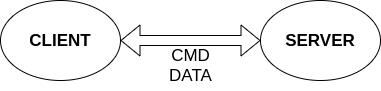
\includegraphics[width=\linewidth]{../diagrams/architettura/1.png}
	\end{subfigure}
	\caption{Single-server}
\end{figure}



\subsection{Virtual server}

\paragraph{} La soluzione single-server può essere migliorata aggiungendo un \emph{livello di virtualizzazione}. Il sistema non viene quindi eseguito direttamente sull'hardware ma all'interno di una \underline{macchina virtuale (VM)}\cite{vm}. 

\paragraph{} La macchina virtuale viene periodicamente \emph{copiata} (interamente o in modo incrementale\cite{backuptypes}) e salvata in un \underline{dispositivo di memorizzazione dedicato}. 

\paragraph{} Nel caso ci fosse un \emph{crash} o \emph{errore critico del sistema operativo}, basta ricaricare la macchina virtuale più recente. La \emph{perdita di dati} è limitata all'età dell'ultimo backup. 

\paragraph{Vantaggi} \begin{itemize}
	\item \emph{Recovery} buona e in tempi brevi in caso di crash.
	\item Naturale implementazione in ambienti di loro natura virtualizzati (es \emph{container}).
\end{itemize}


\paragraph{Svantaggi} \begin{itemize}
	\item Durante il \emph{periodo di transizione} il sistema non risponde.
	\item \emph{Prestazioni} leggermente ridotte a causa della virtualizzazione.
\end{itemize}

\begin{figure}[H]
	\centering
	\begin{subfigure}{0.60\linewidth}
		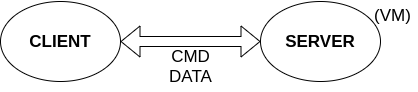
\includegraphics[width=\linewidth]{../diagrams/architettura/2.png}
	\end{subfigure}
	\caption{Single-server con virtualizzazione}
\end{figure}



\subsection{Cloud backup}

\paragraph{} Il backup può essere effettuato nel \underline{cloud}, piuttosto che in un dispositivo dedicato all'interno del datacenter. Inoltre il backup può essere esteso anche ai dati, oltre che al fs. 

\paragraph{Vantaggi} \begin{itemize}
	\item Protezione in caso di \emph{eventi eccezionali}: i dati non risiedono in un unico luogo fisico.
	\item Il provider può fornire ulteriori garanzie di replicazione.
\end{itemize}

\paragraph{Svantaggi} \begin{itemize}
	\item In generale effettuare un backup nel cloud, anche se solo incrementale, richiede un \emph{elevato utilizzo di banda} e \emph{tempi maggiori}.
	\item I \emph{costi} possono essere maggiori.
\end{itemize}

\begin{figure}[H]
	\centering
	\begin{subfigure}{0.80\linewidth}
		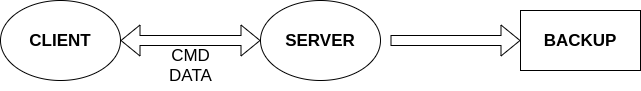
\includegraphics[width=\linewidth]{../diagrams/architettura/3.png}
	\end{subfigure}
	\caption{Aggiunta del backup nel cloud}
\end{figure}



\subsection{Server as distributed database}

\paragraph{} Al posto di utilizzare il filesystem del sistema operativo, è possibile utilizzare un \underline{database distribuito}\cite{ddbms}. Sia metadati che dati vengono \emph{distribuiti automaticamente} nei nodi, garantendo consistenza e fault tolerance. 


\paragraph{Vantaggi} \begin{itemize}
	\item I dati vengono automaticamente replicati e gestiti dal dbms.
	\item Utilizzando un dbms in commercio, si beneficia dall'avere tutto già pronto e costantemente aggiornato.
\end{itemize}


\paragraph{Svantaggi} \begin{itemize}
	\item Maggiore complessità.
	\item La connessione avviene tra il client ed un nodo, il quale poi distribuisce i dati bidirezionalmente agli altri nodi. Inoltre l'utilizzo di banda complessiva può essere doppio rispetto al necessario: nel caso i dati vadano trasferiti dal client al server (gateway) al server di destinazione o vice versa. 
\end{itemize}

\begin{figure}[H]
	\centering
	\begin{subfigure}{0.80\linewidth}
		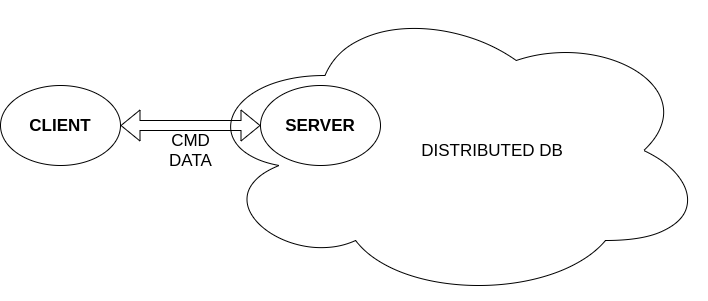
\includegraphics[width=\linewidth]{../diagrams/architettura/4.png}
	\end{subfigure}
	\caption{Utilizzo di un database distribuito}
\end{figure}



\subsection{Meta+Data server}

\paragraph{} L'idea è di far \emph{comunicare direttamente il client con i server in cui verranno memorizzati i dati}. Così facendo si elimina il bottleneck del nodo che prima doveva fungere da "gateway". 

\paragraph{} Un primo sviluppo è quello di \emph{separare i compiti}: si hanno quindi \underline{un} \textbf{meta server} e \underline{uno o più} \textbf{data server}. Il meta server si occupa di memorizzare e gestire il filesystem (metadati), mentre i data server memorizzano soltanto i dati conenuti nei documenti. 

\paragraph{} Per effettuare una qualsiasi \emph{operazione di trasferimento} il client si rivolge inizialmente al meta server, dal quale ottiene la configurazione per contattare il giusto data server e trasferire i dati. Le \emph{operazioni sul filesystem} sono eseguite all'interno del meta server. In questo modo ci sono \emph{due comunicazioni bidirezionali}: client-meta, per la gestione del fs; client-data, per il trasferimento dei dati.

\paragraph{} Per migliorare le prestazioni, soprattutto nel caso in cui il client abbia una banda più ampia rispetto ai data server, i documenti di grandi dimensioni vengono spezzati in \underline{chunks} e distribuiti. 

\paragraph{} Come nel caso single-sever, il meta server è unico, virtualizzato e sottoposto a backup periodico. 

\paragraph{Vantaggi} \begin{itemize}
	\item Trasferimenti concorrenti con data server multipli permettono di migliorare le prestazioni nel caso in cui il client abbia una banda elevata rispetto ai dataserver.
	\item Un \emph{unico meta server} permette di mantenere in modo semplice la consistenza del filesystem.
\end{itemize}

\paragraph{Svantaggi} \begin{itemize}
	\item La frequenza dei \emph{backup} del meta server è fondamentale per minimizzare la perdita di dati in caso di fault.
	\item Tutti i data server devono essere \emph{raggiungibili} dal client (maggiore attenzione alla sicurezza e struttura della rete).
\end{itemize}

\begin{figure}[H]
	\centering
	\begin{subfigure}{0.60\linewidth}
		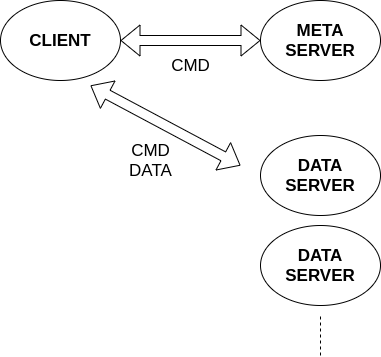
\includegraphics[width=\linewidth]{../diagrams/architettura/5.png}
	\end{subfigure}
	\caption{Separazione di meta e data server}
\end{figure}



\subsection{Meta+Data server 2}

\paragraph{} Facendo dialogare meta e data server, è possibile:\begin{enumerate}
	\item Spostare l'\emph{onere di configurazione dei data server} da client a meta server.
	\item Gestire in qualsiasi momento la \emph{replicazione dei dati}, ad esempio per bilanciare il carico o far fronte alla perdita di un nodo.
	\item Il meta server può monitorare \emph{prestazioni} e \emph{stato di salute} dei data sever.
\end{enumerate}

\paragraph{} Il client quindi si limita a trasferire i dati da/verso data server utilizzando \underline{token} forniti dal meta server. 

\paragraph{Vantaggi} \begin{itemize}
	\item Il sistema può \emph{riconfigurarsi} in ogni momento per far fronte a qualsiasi evenienza.
	\item Ruolo del client semplificato.
	\item Maggiore sicurezza (minore esposizione) perché il client non può inviare comandi ai data server.
\end{itemize}


\paragraph{Svantaggi} \begin{itemize}
	\item Maggiore complessità nel gestire operazioni \emph{concorrenti} ed \emph{asincrone} in nodi diversi.
\end{itemize}

\begin{figure}[H]
	\centering
	\begin{subfigure}{0.60\linewidth}
		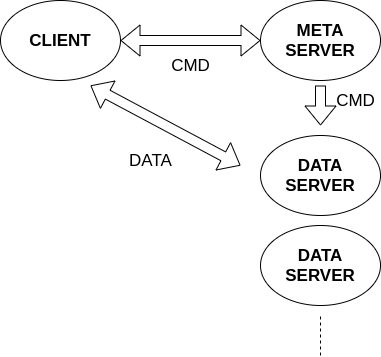
\includegraphics[width=\linewidth]{../diagrams/architettura/6.png}
	\end{subfigure}
	\caption{Meta + data server, il meta server dialoga con i data server}
\end{figure}



\subsection{Meta server as distributed system}

\paragraph{} In questa soluzione non è presente un unico meta server, ma viene utilizzato un sistema distribuito. In generale è preferibile utilizzare un dbms distribuito presente in commercio per gestire i dati a basso livello. 

\paragraph{} Come dimostrato dal teorema CAP bisogna rinunciare alla disponibilità per garantire la coerenza del fs. 

\paragraph{Vantaggi} \begin{itemize}
	\item Possibilità di utilizzo di software in commercio.
	\item Maggiore fault tolerance dei metadati.
	\item Minore tempo di down in caso di malfunzionamenti.
\end{itemize}

\paragraph{Svantaggi} \begin{itemize}
	\item Maggiore difficoltà nell'implementazione dei meta server e dei protocolli di comunicazione tra i vari componenti. 
	\item Maggiore overhead (e quindi minori prestazioni) nel caso di sistemi di piccole/medie dimensioni.
\end{itemize}

\begin{figure}[H]
	\centering
	\begin{subfigure}{0.80\linewidth}
		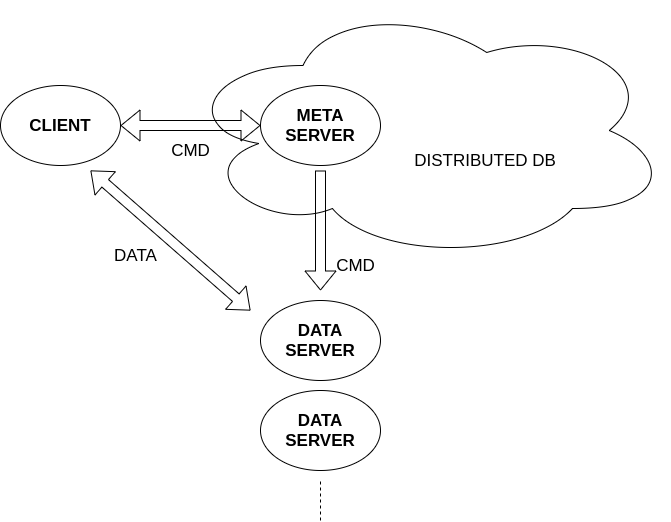
\includegraphics[width=\linewidth]{../diagrams/architettura/7.png}
	\end{subfigure}
	\caption{Il meta server è implementato come database distribuito}
\end{figure}


\section{Struttura del filesytem}

\paragraph{} Il filesystem\cite{fs} ha una struttura non convenzionale. Descriveremo quindi la semantica dei path e i metadati ad essi associati. 

\subsection{Semantica dei path}

\paragraph{} Nei \emph{sistemi tradizionali} il filesystem è formato da \emph{cartelle, file e link}. La \emph{struttura} è ad albero oppure grafo, con o senza la possibilità di cicli. La cartella "base" è root (nei sistemi unix-like denotata con la stringa "/"). Un \emph{path}\cite{path} può essere associato ad uno delle tre tipologie sopra menzionate; il filesystem memorizza questa associazione oltre che ad altri metadati. 

\paragraph{} Il simbolo '/' viene usato per separare i \emph{componenti di un path}: ad esempio il path "/dir1/dir2/file1" identifica il file "file1" figlio della directory "dir2" che a sua volta è figlia della directory "dir1" che è figlia di root. Per questo '/' compare tra i caratteri vietati per la nominazione di un oggetto.  

\paragraph{} Nel \emph{sistema presentato} esistono soltanto i \textbf{documenti}. Essi sono \emph{contenitori di dati}, ed hanno associati alcuni \emph{metadati} (in versione semplificata rispetto a UNIX). 

\paragraph{} Un path che termina con un carattere diverso da '\%' rappresenta un \emph{singolo documento} (es: "documento1", "home/lavoro\#foto/mare-foto1"). Un path che termina con '\%' rappresenta l'\emph{insieme di documenti} che ha come prefisso i caratteri antecedenti al simbolo finale (es. "home/lavoro\#foto\%" include tutti i path che rispettano l'espressione regolare "home/lavoro\#foto*"). Il carattere '\%' può essere usato solo come terminatore. Il carattere ';' è vietato in quanto usato come separatore degli argomenti. 

\paragraph{} Questa organizzazione possiede intrinsecamente una \emph{struttura ad albero}. I path che rappresentano insiemi di documenti sono chiamati \emph{repository}. Le operazioni effettuate su repository hanno effetto su tutti i documenti (anche non ancora creati) appartenenti alla repository. La repository root è naturalmente identificata con il path "\%". "" è un documento valido: si consiglia di usarlo per salvare le informazioni sul sistema (es proprietario, descrizione, contatti) in formato testuale con codifica UTF. 

\subsection{Metadati di un documento}

\paragraph{} I metadati associati ad un documento sono: 

\begin{itemize}
	\item uid: identificatore univoco dell'oggetto, in formato UUID Type 1\cite{uuid};
	\item path: deve rappresentare un documento, stringa UTF\cite{utf};
	\item created: timestamp di creazione in formato UTC\cite{utc};
	\item size: dimensione in byte, 0 per le directory, formato unsigned int;
	\item owner: utente proprietario, stringa UTF;
	\item priority: numero minimo di copie, coincide con la priorità, formato unsigned int;
	\item checksum: checksum sha1, formato esadecimale;
	\item deleted: timestamp di eliminazione (vuoto se non eliminato), formato UTC.
\end{itemize}


\section{Comandi gestiti dal client}

\paragraph{} Di seguito l'elenco e la descrizione dei comandi gestiti dal client, su cui deve basarsi l'implementazione del sistema.

\begin{itemize}
	\item list: lista i metadati di un path (documento o documenti attualmente in una repository);
	
	\item get: download di un documento;
	
	\item push: upload di un documento;
	
	\item rem: eliminazione di path (documento o repository);
	
	\item lock: lock e unlock di un path (documento o repository);
	
	\item setPriority: aggiornare la priorità di un path (documento o repository).
\end{itemize}


\section{Protocollo di comunicazione}

\paragraph{} Il protocollo di comunicazione\cite{comproto} tra nodi diversi si basa sullo scambio di messaggi. Il flusso di dati è binario. Viene utilizzata una connessione di tipo TCP per garantire ordine di consegna, affidabilità, gestione della connessione. 

\paragraph{} Il formato dei comandi è testuale (codifica UTF). Un comando è formato dalla parola chiave che lo identifica e dalla lista degli argomenti. Il separatore utilizzato è il punto e virgola; i comandi sono terminati dal newline.

\paragraph{} Di seguito i flussi di dati coinvolti nelle diverse tipologie di richieste.

\subsection{get}

\paragraph{} La richiesta di tipo \emph{get} richiede il trasferimento in entrata di un documento. 

\paragraph{} Inizialmente il \emph{client} contatta il \emph{meta server}, richiedendo un particolare \emph{documento} (mediante path o uid). Il \emph{meta server} seleziona il \emph{data server} ottimale per gestire la richiesta (deve essere online, contenere la risorsa e non essere sovraccarico). Il \emph{meta server} risponde quindi al client specificando l'uid della risorsa (richiesto per identificarla) e l'indirizzo del \emph{data server} a cui collegarsi. Il \emph{client} si disconnette dal \emph{meta server}.

\paragraph{} Il \emph{client} si connette al \emph{data server} inviando una richiesta \emph{get(uid,start\_pos)}. L'argomento \emph{start\_pos} indica da che byte iniziare a trasferire il documento (indice 0-based). Se la risorsa è disponibile (come dovrebbe essere) il \emph{data server} invia un \emph{ack} seguito dal flusso di dati del documento. Altrimenti risponde con \emph{err} seguito dai dettagli. 

\begin{figure}[H]
	\centering
	\begin{subfigure}{0.80\linewidth}
		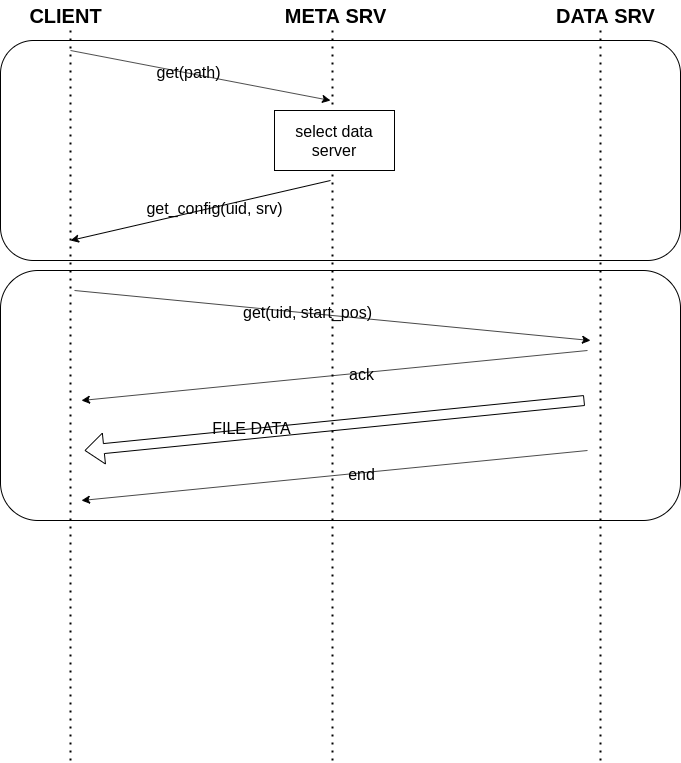
\includegraphics[width=\linewidth]{../diagrams/requests/get_request.png}
	\end{subfigure}
\end{figure}


\subsection{push}

\paragraph{} La richiesta di tipo \emph{push} richiede il trasferimento in uscita di un documento. 

\paragraph{} Inizialmente il \emph{client} contatta il \emph{meta server}, inviando \emph{path} e \emph{size}. Il \emph{meta server} seleziona il \emph{data server} ottimale per gestire la richiesta (deve essere online, poter contenere la risorsa e non essere sovraccarico). Il \emph{meta server} si occupa anche di generare un nuovo \emph{uid} da assegnare alla risorsa. 

\paragraph{} Il \emph{meta server} si collega al \emph{data server} dove verrà inizialmente salvata la risorsa, inviando un comando \emph{create(uid, size)}. Questo comando predispone il \emph{data server} per ospitare un nuovo documento con tale uid e dimensione. Se non ci sono errori, il \emph{data server} risponde al \emph{meta server} con \emph{ack}. Altrimenti con \emph{err} seguito dai dettagli.

\paragraph{} Il \emph{meta server} risponde quindi al client specificando l'uid della risorsa (richiesto per identificarla) e l'indirizzo del \emph{data server} a cui collegarsi. Il \emph{meta server} si disconnette dal \emph{client} e invia le eventuali richieste di eliminazione ai data server (se il documento è una nuova versione di uno esistente).

\paragraph{} Inizia quindi il caricamento del documento. Il \emph{client} si collega al \emph{data server} e invia una \emph{push(uid)}. Se non ci sono errori, il \emph{data server} risponde con \emph{ack} e invia la posizione (indice 0-based) \emph{last\_pos} del primo byte non trasferito (equivalente al numero di byte già trasferiti). A quel punto il \emph{client} trasferisce la porzione rimanente di documento. Al termine del trasferimento, se non ci sono errori, il \emph{data server} risponde con \emph{ack}. La connessione viene chiusa.

\paragraph{} Quando il trasferimento è completato con successo, inizia la terza fase. Il \emph{data server} invia un messaggio del tipo \emph{push\_complete(uid)} al \emph{meta server}. Il meta server inizia quindi ad inviare ai \emph{data server} interessati le richieste di trasferimento, per raggiungere il grado di replicazione voluto.

\begin{figure}[H]
	\centering
	\begin{subfigure}{0.80\linewidth}
		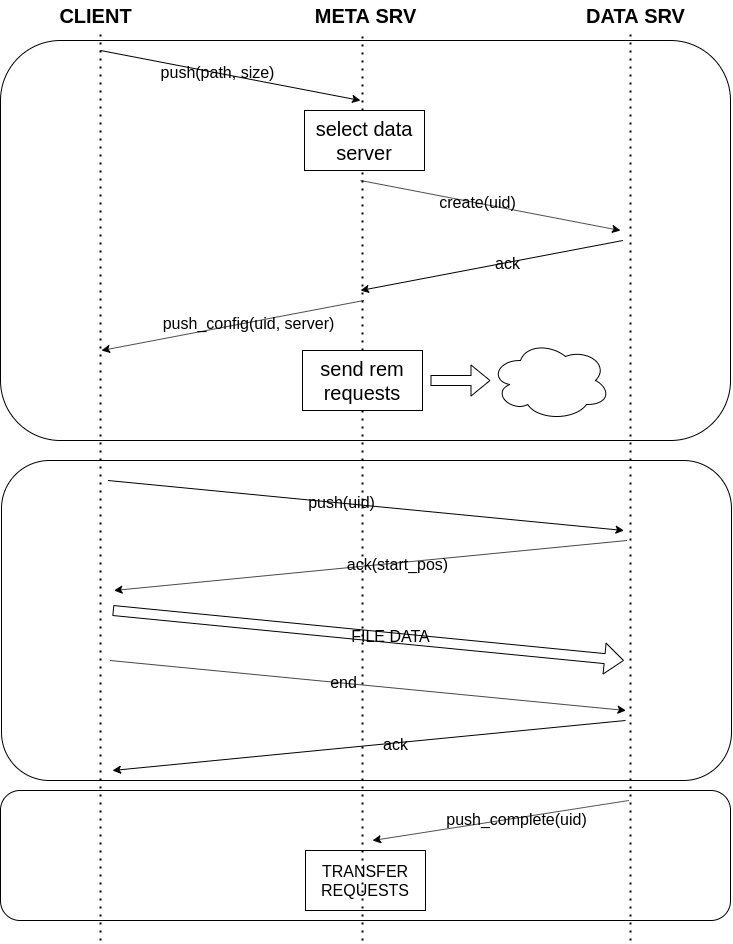
\includegraphics[width=\linewidth]{../diagrams/requests/push_request.png}
	\end{subfigure}
\end{figure}


\subsection{rem}

\paragraph{} La richiesta di tipo \emph{rem} richiede l'eliminazione di un intero path o singolo uid dallo storage.

\paragraph{} Il \emph{client} invia al \emph{meta server} una richiesta \emph{rem}. Se non ci sono errori, il \emph{meta server} risponde con \emph{ack} e chiude la connessione.

\paragraph{} Nel caso la richiesta di eliminazione sia di tipo fisico, il \emph{meta server} contatta separatamente tutti i \emph{data server} contenenti dati relativi a quel particolare \emph{uid} e invia una richiesta \emph{rem(uid)}.  

\begin{figure}[H]
	\centering
	\begin{subfigure}{0.80\linewidth}
		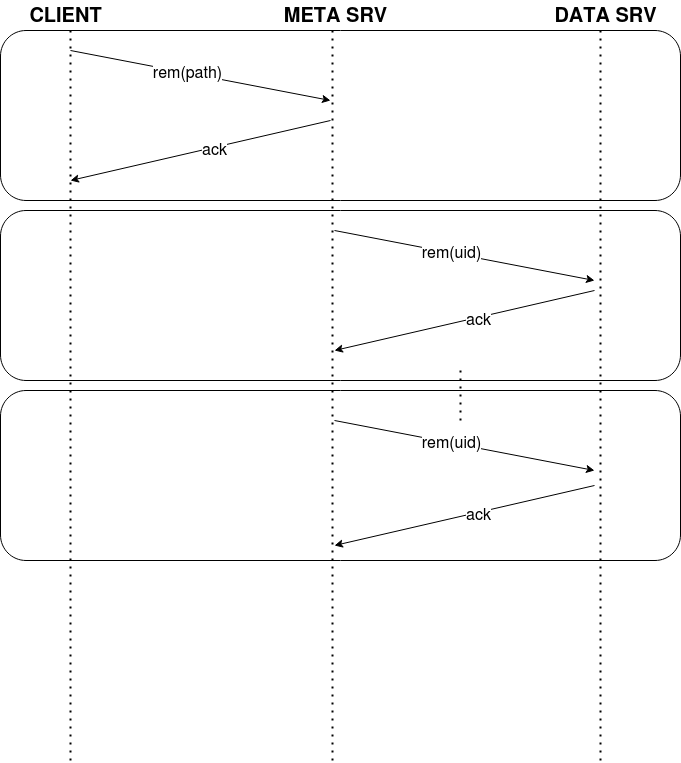
\includegraphics[width=\linewidth]{../diagrams/requests/rem_request.png}
	\end{subfigure}
\end{figure}



\subsection{transfer}

\paragraph{} La richiesta di tipo \emph{transfer}, effettuata esclusivamente dal metaserver, richiede la copia di un documento da un \emph{data server} ad un altro. Viene usata per trasferire i dati tra i nodi in modo da gestire la ridondanza.

\paragraph{} Inizialmente, come nel caso di una \emph{push}, il meta server contatta il \emph{data server} di destinazione (\emph{DATA2}) tramite una richiesta \emph{create(uid)}, per inizializzarlo a ricevere il documento. Se non ci sono errori il \emph{data server} risponde con \emph{ack}. La connessione viene chiusa. 

\paragraph{} A questo punto il \emph{meta server} invia al \emph{data server} di origine (\emph{DATA1}) una richiesta \emph{transfer(uid, to)} per ordinare il trasferimento. Se \emph{DATA1} riesce a connettersi con successo a \emph{DATA2}, risponde a \emph{META} con \emph{begin\_transfer(uid)}. \emph{META1} invia a \emph{META2} una richiesta di tipo \emph{push(uid)} e da luogo al trasferimento. Al termine \emph{DATA1} invia un messaggio \emph{end\_transfer(uid)} a \emph{META} per notificare l'avvenuto trasferimento.


\begin{figure}[H]
	\centering
	\begin{subfigure}{0.80\linewidth}
		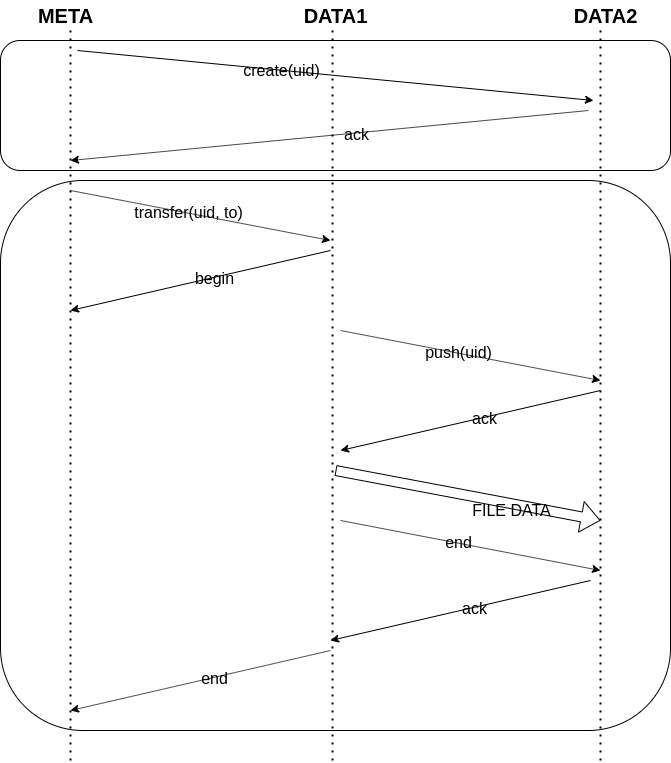
\includegraphics[width=\linewidth]{../diagrams/requests/transfer_request.png}
	\end{subfigure}
\end{figure}



\section{Logging}

\paragraph{} Tutte le operazioni prima di essere eseguite vengono registrate in appositi database di log\cite{logfile}. In questo modo, se un'operazione viene interrotta per qualsiasi motivo, può essere analizzata e rieseguita, in modo da non lasciare spazzatura. 

\paragraph{} Ciò è molto utile anche in fase di debugging/testing: analizzare lo stacktrace ed il flusso di operazioni avvenute precedentemente ad un problema è il modo più efficace per comprenderne le cause. Il modulo \emph{logging}, parte della libreria standard di Python3, permette di organizzare le operazioni di log in modo compatto ed efficace. 


\section{Sicurezza ed autenticazione}

\paragraph{} Tutte le connessioni vengono cifrate a livello intermedio tramite protocollo TLS \cite{tls} over TCP. In questo modo la cifratura è invisibile alla logica dell'application e può in ogni momento essere modificata dal programmatore. Inoltre, essendo una tecnologia ampiamente diffusa e collaudata, presenta una vulnerabilità minima. 

\paragraph{} L'autenticazione da client a server avviene tramite token all'inizio della connessione. La password di ciascun utente può essere cambiata in ogni momento dall'utente stesso, dopo essersi loggato. 

\paragraph{} L'autenticazione da server a server avviene tramite certificato digitale.

\paragraph{} Per garantire sia l'integrità che la sicurezza (per evitare modifiche volute) viene conservato e verificato il checksum (sha1 \cite{sha1}) di tutti i documenti in ingresso. 


\section{Generazione di una chiave identificativa}

\paragraph{} Il problema della generazione di una chiave identificativa\cite{key} è spesso sottovalutato. Consiste nella creazione di un codice che identifichi univocamente una risorsa, un oggetto o un sistema. Questa chiave deve avere la caratteristica di unicità, ovvero non devono esistere codici duplicati: altrimenti non sarebbe più possibile identificare correttamente la risorsa. Inoltre, per ragioni di efficienza, la chiava deve avere lunghezza limitata, in modo da limitarne il tempo di comparazione e lo spazio occupato. In genere le chiavi non hanno un significato, quindi possono essere interpretate indifferentemente come interi o stringhe esadecimali.  

\paragraph{Strategie di generazione di una chiave} Alcune possibili strategie di generazione di chiavi sono: \begin{itemize}
	\item Contatore intero.
	\item Funzione di hash applicata ad un insieme di proprietà variabili con il tempo.
	\item Numero casuale.
	\item UUID.
\end{itemize}

\paragraph{} Il caso più semplice è quello del contatore intero. Solitamente si implementa con un contatore che parte da 0 e viene incrementato di un unità ad ogni generazione. I vantaggi sono: semplicità di implementazione e garanzia di unicità nel contesto del generatore, ovvero il generatore garantisce una sequenza di valori senza duplicati. Questa soluzione può essere implementata efficacemente soltanto all'interno di un sistema che disponga di un solo generatore, quindi di un solo nodo. Inoltre ciò espone all'esterno il numero di chiavi generate sin ora, informazione che potrebbe essere sfruttata per attacchi al sistema. 

\paragraph{} Per superare il problema dell'unicità del nodo una soluzione è prependere al codice l'identificativo del nodo. Ciò garantisce l'unicità della chiave nell'insieme generato dall'intero cluster. È necessario che gli identificativi dei nodi siano univoci, pena il fallimento del sistema. Questo potrebbe essere un problema nel caso venga effettuato un merge tra cluster diversi: se due nodi avevano lo stesso identificativo, almeno uno di essi deve essere rinominato, assieme a tutte le chiavi da esso generate. Ciò potrebbe non essere possibile.  

\paragraph{} Una delle soluzioni più comunemente usate per la generazione di identificativi è l'utilizzo degli \emph{UUID}\cite{uuid}. Gli \textbf{UUID} (Universally Unique Identifier) sono stringhe binarie di 128 cifre generate con precise regole, dipendenti dalla versione. Spesso vengono rappresentati in esadecimale ed compaiono tra i tipi primitivi di molti linguaggi (tra cui CQL).

\paragraph{} Gli UUID di tipo 4 sono generati casualmente. Se viene utilizzato un generatore con distibuzione uniforme, per avere il 50\% di probabilità di registrare almeno una collisione è necessario generare $2.71*10^{18}$ valori. Questa probabilità, seppur non nulla, quasi sempre viene trascurata. Quando però la generazione di un duplicato potrebbe portare il sistema in uno stato inconsistente, è necessario adottare accorgimenti specifici per riportare il sistema ad uno stato safe. 

\paragraph{} Gli UUID di tipo 1, o \emph{TimeUUID}, sono invece generati a partire da istante temporale (UTC), un identificativo del nodo e un numero di sequenza. Come identificativo del nodo si adotta l'indirizzo MAC della scheda di rete del pc, il quale è garantito essere univoco dal costruttore. La presenza dell'istante temporale permette di ordinare gli identificativi per ordine cronologico. L'identificativo del nodo impedisce collisioni tra nodi diversi. Il numero di sequenza elimina le collisioni (fino a $2^{12}$) per elementi generati dallo stesso nodo nello stesso millisecondo: la capacità di generazione garantita è quindi di 4096 UUID tipo 1 al millisecondo. 

\paragraph{} Il problema principale degli UUID tipo 1 è causata dalla presenza di due nodi associati alla medesima scheda di rete, per i quali la probabilità di conflitto è estremamente elevata. Ciò si risolve imponendo l'esecuzione di una sola istanza del software per host, dato un cluster.   


https://tools.ietf.org/html/rfc4122.html


\section{Problema della consistenza in un sistema distribuito}

\paragraph{} I sistemi distribuiti sono per loro natura soggetti a frequenti errori, ritardi di comunicazione e situazioni di concorrenza. È quindi fondamentale assicurarsi di mantenere la consistenza\cite{consistency} dello stato globale in modo che eventuali vincoli di integrità non siano violati. 

\paragraph{} Un esempio lampante è quello delle richieste del tipo "INSERT .. IF NOT EXISTS". Tale operazione non può essere valutata in un solo nodo, in quanto l'identificativo cercato potrebbe essere stato inserito in un altro nodo, ma non ancora propagato all'intero sistema. 

\paragraph{} Per verificare l'esito di tale richiesta è quindi necessario adottare una politica specifica, quale potrebbe essere il meccanismo del \textbf{QUORUM}\cite{quorum}. Essa stabisce che se in un istante la maggioranza assoluta ($Q=floor(N/2) + 1$, con $N$ numero di nodi) dei nodi concorda su una proprietà, allora essa in quell'istante è vera. Capiamo meglio con un esempio: viene inserito il valore 1 all'interno di un nodo. Esso propaga il valore ad almeno $Q-1$ nodi distinti. Al termine dell'operazione almeno la $Q$ nodi contengono il valore 1. Per verificare la presenza del valore 1, viene effettuata una richiesta ad almeno $Q$ nodi distinti qualsiasi. Per il principio della piccionaia, almeno uno di essi conterrà il valore specificato e quindi risponderà "yes", dando il risultato corretto. 

\paragraph{} Il nuovo problema da affrontare è che l'algoritmo precedente vale se e solo se tutte le richieste vengono valutate allo stesso istante, e il risultato ottenuto è garantito solo per lo stesso istante. Questo però è impossibile, in quanto comunicazioni e computazioni non sono istantanee. La soluzione adottata da Cassandra\footnote{Cassandra è il \emph{distributed dbms} impiegato nella mia implementazione, uno tra i più attualmente utilizzati} è l'utilizzo del protocollo \emph{PAXOS}\cite{paxos} per effettuare \emph{Lightweight transactions}\cite{lwt}. Le LWT sono utilizzate in particolare nell'esecuzione di comandi "INSERT $\dots$ IF NOT EXISTS" e "UPDATE ... IF CONDITION", in modo da garantire la consistenza.  

\paragraph{} Inoltre, Cassandra permette di stabilire il livello di consistenza\cite{conslevel} per ogni query di tipo select. Esso può essere ANY, ONE, TWO, THREE, \dots, QUORUM, $\dots$, ALL, in base alle necessità del sistema. Questa scelta consente di bilanciare il tradeoff tra \emph{disponibilità} e \emph{consistenza}. ANY fornisce la maggiore disponibilità (basta che un nodo qualsiasi risponda), ALL la maggiore consistenza (tutti i nodi devono concordare). Per questo progetto è stata scelta l'opzione QUORUM, in quanto garantisce forte consistenza ma tolleranza ai guasti fino a $floor(N)$ nodi. 


\section{Implementazione}

\paragraph{} Di seguito verranno mostrati i punti salienti dell'implementazione demo da me sviluppata. Questa implementazione non è commercializzabile, in quanto incompleta, ma ha lo scopo di provare tutte le funzionalità del sistema sopra descritto. 

\subsection{Strumenti software}

\paragraph{} Il linguaggio scelto per implementare client, dataserver e metaserver è \textbf{Python 3}\footnote{\url{https://www.python.org/download/releases/3.0/}}. Questo linguaggio ha numerosi vantaggi: è \emph{platform-independent}, è \emph{semplice}, \emph{efficace} da utilizzare, permette la scrittura di codice abbastanza \emph{compatto}, possiede una collezione di \emph{librerie} praticamente illimitata, si adatta bene alla programmazione \emph{concorrente}. Unico punto debole è l'\emph{efficienza}, minore rispetto al C++, ma comunque più che sufficiente per lo scopo. 

\paragraph{} Come dbms per il \underline{metaserver} ho scelto \textbf{Apache Cassandra}\footnote{\url{https://cassandra.apache.org/}}, uno dei più famosi sistemi \emph{NoSQL} distribuiti in commercio. Gestisce automaticamente la \emph{replicazione} e \emph{concorrenza} all'interno del cluster, con efficacia, in modo da assicurare \emph{disponibilità} e \emph{affidabilità}. Le \emph{prestazioni} sono ottime, come il supporto della \emph{community} e la \emph{documentazione}. \emph{Cql} (Cassandra Query Language) una sintassi molto simile a SQL, cosa che agevola molto l'intervento di programmatori non specializzati.  

\paragraph{} Dato che i \underline{dataserver} devono essere più leggeri possibile, come dbms per i dataserver ho scelto \textbf{SQLite3}\footnote{\url{https://www.sqlite.org/index.html}}. E' completamente integrato nella libreria standard di Python 3, quindi non necessita dell'installazione di software aggiuntivo. Tutti i dati vengono memorizzati all'interno di un \emph{unico file compresso}. Le \emph{performances} sono più che adatte per le operazioni richieste. Sia buona \emph{documentazione} che \emph{facilità} di utilizzo sono punti a favore. Il linguaggio è un \emph{dialetto SQL}, molto simile a quello degli altri sistemi (l'unica differenza importante sta nei tipi di dato, che sono semplificati).  

\paragraph{} I \emph{file di configurazione} sono in formato \textbf{YAML}\cite{yaml}: un formato \emph{open}, \emph{human-readable} tra i più diffusi al mondo e intuitivi. 


\subsection{Struttura del codice}

\paragraph{} Il codice sia di dataserver che metaserver si articola in 5 parti:\begin{itemize}
	\item Caricamento della cofigurazione.
	\item Interfaccia di connessione e scambio dati.
	\item Interfaccia al database.
	\item Operazioni periodiche.
	\item ServerSocket e relativo handler.
\end{itemize}

\paragraph{} Il client dispone soltanto dell'interfaccia di connessione/scambio dati e dell'implementazione delle operazioni. 

\subsection{Caricamento della configurazione}

\paragraph{} Sia per metaserver che dataserver è obbligatorio fornire il percorso del file di configurazione come primo argomento. 

\subsubsection{Metaserver}

\begin{lstlisting}[language=Python, title=Codice]
if len(sys.argv) > 1:
	configFile = sys.argv[1]
	print("load config", configFile)
	config = yaml.full_load(open(configFile, "r"))
	print("config", config)
else:
	logging.error("Please provide config file")
	exit(1)

database = Database()

for dataserver in config["dataservers"]:
	database.addDataServer(dataserver)
	print("add dataserver", dataserver)
\end{lstlisting}

\begin{lstlisting}[title=Esempio di configurazione]
dataservers:
	- localhost:10010
	- localhost:10011
	- localhost:10012
\end{lstlisting}

\subsubsection{Dataserver}

\begin{lstlisting}[language=Python, title=Codice]
if len(sys.argv) > 1:
	configFile = sys.argv[1]
	print("load config", configFile)
	config = yaml.full_load(open(configFile, "r"))
	print("config", config)
	NAME = config["name"]
	HOST = config["host"]
	PORT = config["port"]
	METASERVER = config["metaserver"]
	workingDir = config["workingDir"]
else:
	logging.error("Please specify config file")
	exit(1)
	
if not os.path.exists(workingDir):
	os.makedirs(workingDir)
	os.chdir(workingDir)
	logging.info("work on %s", os.getcwd())

#create db if not exists
if not os.path.exists("database.db"):
	with sqlite3.connect('database.db') as conn:
		with open("../../dataserver/create_db.sqlite3", "r") as sql:
			conn.executescript(sql.read())

database = Database()
database.setStats(config["storage"], config["downspeed"], config["upspeed"])

SERVER = str(HOST) + ":" + str(PORT)

\end{lstlisting}

\begin{lstlisting}[title=Esempio di configurazione]
name: dataserver10012
workingDir: /home/ale/Dropbox/tesina iot/code/data/dataserver10012
host: localhost
port: 10012
storage: 100000000
downspeed: 50
upspeed: 10
metaserver: localhost:10000
\end{lstlisting}


\subsection{Interfaccia di connessione e scambio dati}

\paragraph{} L'interfaccia è unica per client, metaserver e dataserver. E' implementata come \emph{adapter}\cite{adapter} per la classe socket e StreamRequestHandler. Utilizza gli oggetti \emph{rfile} (lettura) e \emph{wfile} (scrittura), ottenuti dal socket, per effettuare i trasferimenti. 

\paragraph{} Il trasferimento dati avviene in \emph{modalità binaria}, per ragioni di efficienza. 

\paragraph{} I file vengono scritti dal metodo ad alta efficienza \emph{socket.sendfile}, il quale permette di evitare il \emph{double buffering}. Vengono letti a blocchi di 1024 byte con il metodo \emph{socket.read}.

\begin{lstlisting}[language=Python, title=Codice]
def CustomConnection(cls):
    def addrFromString(self, addr):
        ip, port = addr.split(":")
        return (ip, int(port))

    def write(self, *args):
        res = ";".join([str(i) for i in args]).strip() + "\n"
        logging.info("write %s", res)
        self.wfile.write(res.encode())

    def readline(self):
        line = self.rfile.readline().strip().decode().split(";")
        logging.info("readline %s", line)
        return line

    def readFile(self, size, outFile):
        size = int(size)
        pos = 0
        while pos != size:
            chunk = min(1024, size - pos)
            # print("read", chunk, "bytes")
            data = self.rfile.read(chunk)
            outFile.write(data)
            pos += len(data)

    def writeFile(self, filepath, startIndex):
        if type(startIndex) != int:
            startIndex = int(startIndex)
        with open(filepath, "rb") as file:
            self.sendfile(file, startIndex)

    setattr(cls, "writeFile", writeFile)
    setattr(cls, "addrFromString", addrFromString)
    setattr(cls, "readFile", readFile)
    setattr(cls, "write", write)
    setattr(cls, "readline", readline)

    return cls


@CustomConnection
class Connection(socket.socket):
    def __init__(self, endpoint):
        super(Connection, self).__init__(socket.AF_INET, socket.SOCK_STREAM)
        self.connect(self.addrFromString(endpoint))
        self.wfile = self.makefile('wb', 0)
        self.rfile = self.makefile('rb', -1)


@CustomConnection
class DataServerHandler(StreamRequestHandler):
    def sendfile(self, *args, **kwargs):
        self.connection.sendfile(*args, **kwargs)
    
    ...code...

\end{lstlisting}

\subsection{Interfaccia al database}

\paragraph{} Per interfacciarsi al database metaserver e dataserver hanno degli oggetti dedicati, chiamati \emph{Database}. Essi espongono tutte le query sotto forma di \emph{API}: in questo modo gli utilizzatori del database sono svincolati dall'effettiva implementazione sottostante. Questo è un vantaggio sia in termini di \emph{incapsulamento}, che rende più semplice la progettazione e manutenzione del software, che nel caso in cui si voglia cambiare dbms, perché l'utilizzatore non deve essere modificato. 

\subsubsection{Metaserver}

\paragraph{} Di seguito la struttura del database utilizzato dal metaserver assieme ad una parte di implementazione dell'oggetto Database. 


\begin{lstlisting}[language=SQL, title=Struttura]
--il fattore di replicazione deve essere <= al numero di server a disposizione
create keyspace metaserver with replication = {'class' : 'SimpleStrategy', 'replication_factor' : 1};


use metaserver;


/*un metaserver*/
create table dataserver(
	server text,      --indirizzo in formato host:port del dataserver
	online boolean,     --se in questo momento (all'ultima rilevazione) e' online
	capacity bigint,     --capacita' in byte totale
	remaining_capacity bigint,     --capacita' in byte disponibile (totale-utilizzata)
	available_down float,     --banda in Mb/s disponibile per il download
	available_up float,       --banda in Mb/s disponibile per l'upload
	primary key(server)
);

/*un documento*/
create table object(
    uid uuid,
    path text,        --path associato al documento
    created timestamp,     --istante di creazione (nel metaserver)
    owner text,     --proprietario (colui che l'ha creato)
    size bigint,     --dimensione in byte
    priority int,     --livello di priorita' (di replicazione)
    checksum text,      
    deleted timestamp,       --istante di eliminazione (NULL se non eliminato)
    primary key(uid)
);

/*lock attivi*/
create table object_lock(
    path text,    --path del documento
    user text,      --utente che detiene il lock
    primary key(path)
);

/*log delle performance dei dataserver*/
create table performance_log(
    server text,           --indirizzo del dataserver nel formato host:port
    time timestamp,     --istante di registrazione del record
    online boolean,         
	capacity bigint,
	remaining_capacity bigint,
	available_down float,
	available_up float,
	primary key(server, time)
);

/*oggetti che vanno verificati*/
create table pending_object(
    uid uuid,           --uid dell'oggetto
    enabled boolean,       --se false, l'oggetto non puo essere attualmente processato perche' non e' disponibile o non sono disponibili server in cui replicarlo
    primary key(uid)
);

/*documenti salvati nei dataserver*/
create table stored_object(
    uid uuid,       --documento
    server text,       --indirizzo del server in cui e' salvato, nel formato host:port
    created timestamp,
    complete boolean,
    primary key(uid, server)
);

/*utilizzato per le ricerche di prefissi del tipo "where path like '<prefix>%'"*/
create custom index object_path_idx on object(path)
using 'org.apache.cassandra.index.sasi.SASIIndex';

/*utilizzato per selezionare l'ultima versione di un documento, dato il path (con cql non e' possibile ordinare nella query) */
create materialized view pathToObject as select * from object where path is not null
primary key (path, uid)
with clustering order by (uid desc);


\end{lstlisting}


\begin{lstlisting}[language=Python, title=Codice]
class Database:
    def __init__(self):
  		#livello di consistenza delle query
        profile = ExecutionProfile(
            consistency_level=ConsistencyLevel.QUORUM,
            serial_consistency_level=ConsistencyLevel.SERIAL  #LWT
        )
		
		#connessione al cluster
        self.cluster = Cluster(protocol_version=4, execution_profiles={EXEC_PROFILE_DEFAULT: profile})
        self.session = self.cluster.connect("metaserver")

	#aggiunta di un nuovo dataserver. inizialmente stato=disconnesso
    def addDataServer(self, addr):
        self.session.execute("insert into dataserver(server, online) values (%s, false)", (addr, ))

	#creazione di un nuovo documento
    def addObject(self, uid, path, owner, size, priority, checksum):
        created = datetime_from_uuid1(uid)  #l'istante di creazione del documento coincide con l'istante di creazione del suo uid
        
        self.session.execute("insert into object(uid, path, created, owner, size, priority, checksum) "
                             "values (%s, %s, %s, %s, %s, %s, %s)"
                             , (uid, path, created, owner, size, priority, checksum))
        return uid

	#una nuova copia fisica di un documento viene creata in un dataserver
    def addStoredObject(self, uid, server, complete=False, created=None):
        if created is None: created = datetime.now() #istante di creazione della replica, non del documento
        
        self.session.execute("insert into stored_object(uid, server, created, complete) values (%s, %s, %s, %s)",
                             (uid, server, created, complete))
        return id

	#effettua il lock di un path (singolo documento)
    def lockPath(self, path, user="root"):
    	#se il path che si intende bloccare e' gia' presente nella tabella, il constraint INSERT IF NOT EXISTS fallisce e applied viene settato a False (altrimenti True)
        return self.session.execute("insert into object_lock(path, user) values (%s, %s) if not exists",
                                    (path, user)).one().applied

	#unlock di un path
    def unlockPath(self, path):
        self.session.execute("delete from object_lock where path = %s", (path, ))

	#ottiene lo stato di lock di un path e l'identificativo dell'utente che detiene il lock (se bloccato, altrimenti "")
    def getPathLock(self, path):
        r = self.session.execute("select * from object_lock where path = %s", (path, )).one()
        
        if r is None:    #none se non presente nel db l'entry relativa al path specificato (quindi e' sbloccato)
            return False, ""
        else:
            return True, r.user

	#ottiene i metadati di un documento dato l'uid
    def getObjectByUid(self, uid):
        return self.session.execute("select * from object where uid = %s", (uid, )).one()

	#lista di tutti i documenti appartenenti ad un determinato path (singolo o repository)
    def list(self, path):
        if path == "" or path == '%':
            return self.session.execute("select * from object").all()
        else:
            return self.session.execute("select * from object where path like %s", (path, )).all()

	#lista dei dataserver
    def getDataServers(self, onlyOnline=True):
        if onlyOnline:   #solo i dataserver online (secondo l'ultima rilevazione)
            return self.session.execute("select * from dataserver where online=true allow filtering").all()
        return self.session.execute("select * from dataserver").all()

    #update dello status di un dataserver (ottenuto a seguito di una rilevazione)
    def updateDataServerStatus(self, addr, online, remaining_capacity=0, capacity=0, available_down=.0, available_up=.0):
        self.session.execute("update dataserver "
                             "set capacity=%s, remaining_capacity=%s, available_down=%s, "
                             "available_up=%s, online=%s where server=%s",
                             (capacity, remaining_capacity,
                              available_down, available_up, online, addr))
        #performances dei dataserver loggate per eventuali analisi
        self.session.execute("insert into performance_log(server, time, capacity, remaining_capacity, available_down,"
                             "available_up, online) values (%s, %s, %s, %s, %s, %s, %s)",
                             (addr, datetime.now(), capacity, remaining_capacity,
                              available_up, available_down, online))

    #rimuove una replica fisica di un documento
    def removeStoredObject(self, uid, server):
        self.session.execute("delete from stored_object where uid = %s and server = %s", (uid, server))

    #rimuove un documento dato l'uid
    def removeObject(self, uid):
        self.session.execute("delete from object where uid = %s", (uid, ))

    #ottiene la lista di dataserver che contengono l'uid specificato
    def getServersForUid(self, uid, complete=True, online=True):
        if complete:   #solo dataserver la cui replica e' completa (trasferita completamente e validata)
            res = self.session.execute(
                "select server from stored_object where uid = %s and complete = true allow filtering", (uid, )).all()
        else:
            res = self.session.execute(
                "select server from stored_object where uid = %s allow filtering", (uid, )).all()
        if online:  #solo dataserver online (secondo ultima rilevazione)
            def f(srv):
                return self.session.execute("select online from dataserver where server = %s", (srv.server, )).one().online
            res = list(filter(f, res))
        return res

    #testa se un dataserver e' online
    def isServerOnline(self, server):
        return self.session.execute("select online from dataserver where server = %s", (server, )).one().online

    #setta una replica di un documento come completa
    def setComplete(self, uid, server):
        self.session.execute("update stored_object set complete = true where uid = %s and server = %s", (uid, server))

    #marca come eliminato l'ultimo uid (in ordine di creazione) relativo ad un path singolo specificato.
    def markDeleted(self, path):
        res = self.getUidForPath(path)
        timestamp = datetime.now()
        if res is not None:
            self.session.execute("update object set deleted = %s where uid = %s",
                                 (timestamp, res.uid))

    #marca come eliminato uno specifico uid
    def markUidDeleted(self, uid):
        timestamp = datetime.now()
        self.session.execute("update object set deleted = %s where uid = %s",
                             (timestamp, uid))

    #ottiene l'uid dell'ultima versione del documento relativo ad un path singolo
    def getUidForPath(self, path):
        path = str(path)
        return self.session.execute("select * from pathToObject where path = %s", (path, )).one()

    #ottiene la lista di tutti gli uid relativi ad un path singolo (tutte le versioni di un documento)
    def getUidsForPath(self, path):
        return self.session.execute("select * from object where path like %s", (path, )).all()

    #gli uid di tutti i documenti che hanno una replica all'interno del dataserver specificato
    def getUidsForServer(self, server):
        return self.session.execute("select uid from stored_object where server = %s allow filtering", (server, ))

    #aggiunge un uid alla lista di quelli da verificare (per azioni periodiche)
    def addPendingUid(self, uid):
        self.session.execute("insert into pending_object(uid, enabled) values (%s, True)", (uid, ))

    #aggiorna la priorita' di un documento (dato l'uid)
    def updatePriority(self, uid, priority):
        self.session.execute("update object set priority=%s where uid=%s", (priority, uid))

    #lista di tutti gli uid pendenti
    def getPendingUids(self, onlyEnabled=True):
        if onlyEnabled:  #solo quelli attivi
            return self.session.execute("select uid from pending_object where enabled=True allow filtering").all()
        return self.session.execute("select uid from pending_object").all()

    #disabilita un uid pendente. utilizzato ad esempio quando un documento va replicato ma non ci sono dataserver disponibili.
    def disablePendingUid(self, uid):
        self.session.execute("update pending_object set enabled=False where uid = %s", (uid, ))

    #rimuove un uid pendente
    def removePendingUid(self, uid):
        self.session.execute("delete from pending_object where uid = %s", (uid, ))


database = Database()
\end{lstlisting}



\subsubsection{Dataserver}

\paragraph{} Di seguito struttura e implementazione del database relativo ai dataserver.

\begin{lstlisting}[language=SQL, title=Struttura]

--un oggetto
create table object(
    uid text primary key,
    local_path text,   --percorso del file system dov'e' salvato
    size integer,   --dimensione in byte (totale)
    complete integer,    --true se e' completo, false se deve ancora essere totalmente trasferito
    created text,       --istante di creazione (nel dataserver)
    checksum text
);

--configurazione del dataserver
create table stats(
    storage int,        --storage totale in byte
    downspeed int,      --banda totale in download, in Mb/s
    upspeed int         --banda totale in upload, in Mb/s 
);

--documenti che vanno eliminati
create table toBeDeleted(
    uid text primary key        --uid del documento
);


\end{lstlisting}

\begin{lstlisting}[language=Python, title=Codice]
class Database:
    def __init__(self):
        try:
            #connessione al database
            self.connection = sqlite3.connect('database.db')
            self.cursor = self.connection.cursor()

        except sqlite3.Error as error:
            print("error while connecting to database", error)

    #ottiene i metadati relativi ad un documento, dato l'uid
    def getObject(self, uid):
        return self.cursor.execute("select * from object where uid = ?", (str(uid), )).fetchone()

    #elimina i dati relativi ad un documento
    def deleteUid(self, uid):
        self.cursor.execute("delete from object where uid = ?", (uid, ))
        self.cursor.execute("delete from transfer where uid = ?", (uid, ))
        self.cursor.execute("delete from toBeDeleted where uid = ?", (uid, ))
        self.connection.commit()

    #lista di tutti i documenti (anche non completi)
    def getStoredData(self):
        return self.cursor.execute("select uid, created, complete from object").fetchall()

    #spazio complessivo riservato ai documenti attualmente salvati (per i documenti parziali si conta comunque la dimensione totale)
    def reservedSpace(self):
        res = self.cursor.execute("select sum(size) from object").fetchone()[0]
        if res is None:
            res = 0
        return res

    #aggiunge un documento alla coda di eliminazione
    def addToBeDeleted(self, uid):
        self.cursor.execute("insert into toBeDeleted(uid) values (?)", (uid, ))
        self.connection.commit()

    #ottiene tutti i documenti in coda di eliminazione
    def getToBeDeleted(self):
        return self.cursor.execute("select * from toBeDeleted").fetchall()

    #crea una nuova replica di un documento
    def addObject(self, uid, local_path, size, checksum):
        complete = 0
        created = datetime.now()

        self.cursor.execute("insert into object(uid, local_path, size, complete, checksum, created) values (?, ?, ?, ?, ?, ?)",
                            (uid, local_path, size, complete, checksum, created))
        self.connection.commit()

        return self.cursor.lastrowid   #primary key dell'entry inserita

    #setta un documento come completo
    def setComplete(self, uid):
        self.cursor.execute("update object set complete=1 where uid = ?", (uid, ))
        self.connection.commit()

    #ottiene le impostazioni del nodo (banda, capacita', ecc)
    def nodeStats(self):
        return self.cursor.execute("select * from stats").fetchone()

    #modifica le impostazioni del nodo
    def setStats(self, storage, downspeed, upspeed):
        self.cursor.execute("delete from stats")
        self.cursor.execute("insert into stats(storage, downspeed, upspeed) values (?, ?, ?)",
                            (storage, downspeed, upspeed))
        self.connection.commit()

database = Database()
\end{lstlisting}


\subsection{Operazioni periodiche}

\paragraph{} Le operazioni che non possono essere eseguite subito (es: eliminazione di un documento mentre sta venendo trasferito) oppure che vanno eseguite regolarmente (es: monitoraggio delle prestazioni del dataserver) sono valutate \emph{periodicamente} ed eseguite nel primo momento utile. 

\paragraph{} Lo schema di esecuzione è molto semplice: ogni operazione periodica è \emph{schedulata ad intervalli regolari} (es 10 secondi) e viene eseguita da un \emph{looper thread}.

\subsubsection{Metaserver}

\paragraph{} Nel metaserver le operazioni periodiche sono:\begin{itemize}
	\item Controllo dello stato dei dataserver.
	\item Mantenimento del grado di replicazione dei documenti.
\end{itemize}

\begin{lstlisting}[language=Python, title=Controllo dello stato dei dataserver]
def onDataServerConnect(addr):
    print("server", addr, "connected")

    for elem in database.getUidsForServer(addr):
        database.addPendingUid(elem.uid)

    for elem in database.getPendingUids(onlyEnabled=False):
        database.addPendingUid(elem.uid)

def onDataServerDisconnect(addr):
    database.updateDataServerStatus(addr, False)

    for elem in database.getUidsForServer(addr):
        database.addPendingUid(elem.uid)

    print("server", addr, "disconnected")


def checkDataServerStatus(addr):
    wasOnline = database.isServerOnline(addr)   #status dell'ultima rilevazione
    
    try:
        with Connection(addr) as conn:  #richiesta dello status al dataserver
            conn.write("status")
            res = conn.readline()

        status, reservedCapacity, totCapacity, downSpeed, bandDown, upspeed, bandUp = res
       	
        database.updateDataServerStatus(addr, True, totCapacity - reservedCapacity, totCapacity,
                                        downSpeed - bandDown, upspeed - bandUp)

        if not wasOnline:
            onDataServerConnect(addr)
    except ConnectionRefusedError as err:  #accade quando il dataserver non e' raggiungibile
        if wasOnline:
            onDataServerDisconnect(addr)

def monitorDataServers():
    for server in database.getDataServers(onlyOnline=False):
        checkDataServerStatus(server.server)
\end{lstlisting}

\begin{lstlisting}[language=Python, title=Mantenimento del grado di replicazione dei documenti]
def processPendingUids():
    for elem in database.getPendingUids():
        processPendingUid(database, elem.uid)

def processPendingUid(database, uid):
	#metadati dell'uid
    res = database.getObjectByUid(uid)  
    
    priority = res.priority
    size = res.size
    checksum = res.checksum
    
    #repliche attualmente disponibili (solo online)
    serversContaining = {x.server for x in database.getServersForUid(uid)}
    numCopies = len(serversContaining)

    if numCopies == priority:  #se la priorita' coincide con il numero di repliche disponibili non serve fare nulla
        database.removePendingUid(uid)
        return

	#server liberi per ricevere una nuova replica 
	availableServers = [x.server for x in database.getDataServers() if x.server not in serversContaining and x.remaining_capacity > size]
	
	serversContaining = list(serversContaining)

    if numCopies > priority:  #se il numero di copie disponibili supera la priorita' bisogna eliminarne una
        random.shuffle(serversContaining)
        target = serversContaining[0]

        print("remove", uid, "target", target)

        try:
            with Connection(target) as conn:  #invia richiesta di eliminazione al dataserver
                conn.write("deleteUid", uid)
                print(conn.readline())

            database.removeStoredObject(uid, target)  #eseguito solo se la richiesta di eliminazione (connessione) ha avuto successo
        except:
            pass

        return

    if numCopies < priority:   #non ci sono abbastanza copie disponibili

        if len(serversContaining) == 0 or len(availableServers) == 0:   #se non ci sono sorgenti o destinazioni disponibili bisogna attendere
            database.disablePendingUid(uid)
            return

        try:
	        #scegli una sorgente ed una destinazione
	        random.shuffle(availableServers)
	        random.shuffle(serversContaining)
            source = serversContaining[0]
            target = availableServers[0]

            database.addStoredObject(uid, target) #crea una nuova replica

            def process():
                try:
                    with Connection(target) as conn:  #crea il documento sul server di destinazione
                        conn.write("createUid", uid, size, checksum)
                        print(conn.readline())

                    with Connection(source) as conn:   #ordina il trasferimento
                        conn.write("transfer", uid, target)
                        print(conn.readline())
                except:
                    database.removeStoredObject(uid, target) #la replica non e' stata creata con successo
                    database.addPendingUid(uid)

            _thread.start_new_thread(process)  #l'operazione, essendo lunga, viene eseguita su un thread separato

        except:
            print("ERROR")
\end{lstlisting}

\begin{lstlisting}[language=Python, title=Scheduling ed esecuzione]
schedule.every(5).seconds.do(monitorDataServers)
schedule.every(5).seconds.do(processPendingUids)
schedule.run_all()

def repeatedActions(_):
    while True:
        schedule.run_pending()
        time.sleep(0.1)

_thread.start_new_thread(repeatedActions, (None,))
\end{lstlisting}


\subsubsection{Dataserver}

\paragraph{} Nel dataserver le operazioni periodiche sono:\begin{itemize}
	\item Controllo dello \emph{stato interno} (utilizzo della banda e della memoria di massa).
	\item Eliminazione dei documenti in coda.
\end{itemize}


\begin{lstlisting}[language=Python, title=Controllo dello stato interno]
#bandup and banddown in MB/s
performances = {"sent": 0, "recv": 0, "lastTime" : 0, "bandup" : 0, "banddown" : 0}

def getPerformance():
    res = psutil.net_io_counters()
    curtime = time.time()
    delta = curtime - performances["lastTime"]
    performances["lastTime"] = curtime
    performances["bandup"] = (res.bytes_sent - performances["sent"]) / delta / 1000000
    performances["banddown"] = (res.bytes_recv - performances["recv"]) / delta / 1000000
    performances["sent"] = res.bytes_sent
    performances["recv"] = res.bytes_recv
\end{lstlisting}


\paragraph{} Per tenere traccia dei documenti attualmente in trasferimento, che quindi non possono essere eliminati, viene utilizzato il set \emph{processing}. Esso contiene in ogni momento tutti gli \emph{uid} relativi a documenti in caricamento e in trasferimento. 

\begin{lstlisting}[language=Python, title=Eliminazione dei documenti in coda]
def processDeleteUids():

    database = Database()
    uids = database.getToBeDeleted()

    with processingLock:
        for uid, in uids:
            if uid not in processing:
                uid, localPath, size, complete, created, checksum = database.getObject(uid)
                
                if os.path.exists(localPath): os.remove(localPath)
                database.deleteUid(uid)
\end{lstlisting}

\begin{lstlisting}[language=Python, title=Scheduling ed esecuzione]
schedule.every(5).seconds.do(getPerformance)
schedule.every(15).seconds.do(processDeleteUids)

def runPeriodicTasks(_):
    while True:
        schedule.run_pending()
        time.sleep(0.1)

_thread.start_new_thread(runPeriodicTasks, (None,))
\end{lstlisting}


\subsection{ServerSocket e relativo handler}

\paragraph{} Il punto di contatto di metaserver è il metodo \emph{handle}. Esso si occupa del \emph{dispatching delle richieste}, con l'ausilio di una mappa delle operazioni. Si ricorda che, secondo il protocollo di comunicazione, una richiesta è formata dal nome ed eventuali parametri, separati dal punto e virgola e terminati da newline. Una soluzione analoga è presente per il dataserver.

\paragraph{} Una eventuale \emph{richiesta non riconosciuta} viene automaticamente scartata.

\begin{lstlisting}[language=Python, title=Metaserver e relativo handler]
    ...
    
    def handle(self):
        self.database = Database()

        switcher = {
            "getPath": self.getPath,
            "pushPath": self.pushPath,
            "list": self.list,
            "pushComplete": self.pushComplete,
            "test": self.test,
            "deletePath": self.deletePath,
            "addDataServer": self.addDataServer,
            "getUid": self.getUid,
            "lockPath": self.lockPath,
            "getPathLock": self.getPathLock,
            "unlockPath": self.unlockPath,
            "updatePriorityForPath": self.updatePriorityForPath,
            "updatePriorityForUid": self.updatePriorityForUid,
            "permanentlyDeletePath": self.permanentlyDeletePath
        }

        print("handle request from " + str(self.client_address))

        data = self.readline()

        switcher[data[0]](data[1:])

with MetaServer((HOST, PORT), MetaServerHandler, bind_and_activate=True) as server:
    server.serve_forever()
\end{lstlisting}

\paragraph{} In questa sezione vengono analizzate le implementazioni di tutti i metodi/operazioni che possono essere eseguite. L'analisi è suddivisa per operazioni, in modo da poter apprezzare meglio le interazioni tra i componenti. 

\subsubsection{Caricamento di un documento}

\paragraph{} Questa azione viene usata dal client per caricare un documento.

\paragraph{} Inizialmente il client si collega al dataserver inviando \emph{path, dimensione, checksum, priorità, utente}.

\begin{lstlisting}[language=Python, title=Client]
def sendFile(localPath = "small_file.txt", remotePath="testfile.txt", priority=1, user="default"):
    with Connection(METASERVER) as conn:
        size = getsize(localPath)
       
        checksum = hashFile(localPath)

        conn.write("pushPath", remotePath, size, checksum, priority, user)
        res = conn.readline()

        if res[0] != "ok":
            print("ERR", res)
            return False

        state, uid, addr = res
    ...
\end{lstlisting}

\paragraph{} Il metaserver controlla che il path non sia bloccato da un altro utente, cerca un dataserver che possa ospitare il documento e gli assegna un nuovo uid.

\begin{lstlisting}[language=Python, title=Metaserver]
def pushPath(self, args):
    path, size, checksum, priority, user = args
    size = int(size)

    lock, lockUser = self.database.getPathLock(path)
    if lock and lockUser != user:
        self.write("err", "path locked by " + lockUser)
        return False

    dataservers = [x for x in self.database.getDataServers() if x.remaining_capacity > size]

    if len(dataservers) == 0:
        self.write("err", "no data servers available")
        return False

    random.shuffle(dataservers)
    target = dataservers[0]

    uid = uuid4()
    addr = target.server
    ...
\end{lstlisting}

\paragraph{} Il metaserver contatta il dataserver di destinazione creando la risorsa.

\begin{lstlisting}[language=Python, title=Metaserver]
    ...
    with Connection(addr) as dataServer:
        dataServer.write("createUid", uid, size, checksum)
        response = dataServer.readline()

    if response[0] != "ok":
        self.write("err", response)
        return False
    ...
\end{lstlisting}

\begin{lstlisting}[language=Python, title=Dataserver]
def createUid(self, args):
	uid, size, checksum = args
	local_path = os.getcwd() + "/" + uid
	
	with processingLock:
		totCapacity, downSpeed, upspeed = self.database.nodeStats()
		reservedCapacity = self.database.reservedSpace()
		
		if reservedCapacity + size > totCapacity:
			self.write("err", "storage capacity exceeded")
			return False
		
		self.database.addObject(uid, local_path, size, checksum)
		
	self.write("ok")
\end{lstlisting}

\paragraph{} Il metaserver marca come eliminato l'oggetto associato al path (se esiste) e aggiunge il nuovo oggetto al database. Risponde al client indicando \emph{uid, addr}. 

\begin{lstlisting}[language=Python, title=Metaserver]
    self.database.markDeleted(path)
    self.database.addObject(uid, path, "root", size, priority, checksum)
    self.database.addStoredObject(uid, addr)

    self.write("ok", uid, addr)
\end{lstlisting}

\paragraph{} Il client si collega al dataserver target e invia il documento. Se il documento era stato già parzialmente caricato nel dataserver (es. file di grosse dimensioni), il caricamento riprende da dover era rimasto. Se il documento era già stato caricato completamente (ovvero il client tenta di caricare un documento già completo), viene generato un errore. Se il checksum al termine del caricamento non corrisponde, il documento viene subito eliminato per essere ricaricato in futuro. 

\begin{lstlisting}[language=Python, title=Client]
    ...
    with Connection(addr) as conn:
        conn.write("pushUid", uid)

        res = conn.readline()
        if res[0] != 'ok':
            print(res)
            return False

        status, startIndex = res

        print("send starting from", int(startIndex))

        conn.writeFile(localPath, startIndex)
        print(conn.readline())
\end{lstlisting}

\begin{lstlisting}[language=Python, title=Dataserver]
def pushUid(self, args):
    uid, = args

    with processingLock:
        objinfo = self.database.getObject(uid)

        if objinfo is None:
            self.write("ERR", "uid info not found")
            return False

        uid, localpath, size, complete, created, checksum,  = objinfo

        if complete:
            self.write("err", "file complete")
            return False

        processing.add(uid)

    startIndex = 0
    if os.path.exists(localpath):
        startIndex = os.path.getsize(localpath)

    assert startIndex < size   #altrimenti sarebbe complete

    self.write("ok", startIndex)

    with open(localpath, "a+b") as out:
        self.readFile(size - int(startIndex), out)

    file_checksum = hashFile(localpath)

    with processingLock:
        processing.remove(uid)

        print("checksum", checksum, "file_checksum", file_checksum)

        if file_checksum != checksum:
            os.remove(localpath)
            self.write("err", "checksum do not match")
            return False

        self.database.setComplete(uid)
\end{lstlisting}

\paragraph{} Il dataserver invia al metaserver la notifica che il caricamento è completo, e quindi il documento può essere utilizzato.

\begin{lstlisting}[language=Python, title=Dataserver]
    ...
    with Connection(METASERVER) as metaConn:
        metaConn.write("pushComplete", uid, SERVER)

    self.write("ok")
\end{lstlisting}

\paragraph{} Il metaserver processa l'elemento per controllarne il grado di replicazione.

\begin{lstlisting}[language=Python, title=Metaserver]
def pushComplete(self, args):
    uid, addr = args

    self.database.setComplete(uid, addr)
    self.database.addPendingUid(uid)

    self.write("ok")
\end{lstlisting}


\subsubsection{Trasferimento di un documento}

\paragraph{} Il trasferimento viene usato dal metaserver per copiare un documento da un dataserver ad un altro, aumentandone così il grado di replicazione.

\paragraph{} Il metaserver prima configura il server di destinazione per ricevere il documento, come nel caso del caricamento da parte del client. Poi invia la richiesta di trasferimento al server sorgente specificando \emph{uid, indirizzo server destinazione}.

\begin{lstlisting}[language=Python, title=Metaserver]
with Connection(target) as conn:
    conn.write("createUid", uid, size, checksum)
    print(conn.readline())

with Connection(source) as conn:
    conn.write("transfer", uid, target)
    print(conn.readline())
\end{lstlisting}

\paragraph{} Il caricamento del documento dal server sorgente a destinazione avviene con lo stesso metodo usato nel caricamento da client a dataserver.

\begin{lstlisting}[language=Python, title=Dataserver sorgente]
def transfer(self, args):
    uid, server = args

    with processingLock:
        res = self.database.getObject(uid)
        if res is None:
            self.write("err", "uid not found")
            return False

        processing.add(uid)

    uid, localPath, size, complete, created, checksum = res

    with Connection(server) as target:
        target.write("pushUid", uid)
        status, startIndex = target.readline()
        target.writeFile(localPath, startIndex)

    with processing:
        processing.remove(uid)

    self.write("ok")
\end{lstlisting}



\subsubsection{Scaricamento sul client di un documento (dato il path)}

\paragraph{} Questa è l'operazione con cui il client ottiene un documento dal sistema di storage.

\paragraph{} Inizialmente il client contatta il metaserver indicando il path che vuole scaricare.

\begin{lstlisting}[language=Python, title=Client]
def get(localPath = "testin.txt", remotePath = "ale/file1", newFile=True, user="default"):
    if newFile and os.path.exists(localPath):
        os.remove(localPath)

    with Connection(METASERVER) as conn:
        conn.write("getPath", remotePath, user)
        res = conn.readline()

    if res[0] != 'ok':
        print("ERR", res)
        return False

    status, uid, addr, checksum = res
\end{lstlisting}

\paragraph{} Il metaserver verifca che il path non sia bloccato da un altro utente, cerca l'uid associato al path (quello che corrisponde all'ultima versione del documento), cerca un dataserver che lo contenga (possibilmente seleziona il migliore) e risponde al client indicando \emph{uid, indirizzo dataserver}.

\begin{lstlisting}[language=Python, title=Metaserver]
def _getServerForUid(self, uid):
	res = self.database.getServersForUid(uid)
	
	if len(res) == 0:
		self.write("err", "no copies available")
		return False
	
	random.shuffle(res)
	
	addr = res[0].server
	return addr	

def getPath(self, args):
    path, user = args

    lock, lockUser = self.database.getPathLock(path)
    if lock and lockUser != user:
        self.write("err", "path locked by " + lockUser)
        return False

    res = self.database.getUidForPath(path)

    if not res:
        self.write("err", "path not found")
        return False

    if res.deleted is not None:
        self.write("err", "path deleted")
        return False

    uid, checksum = res.uid, res.checksum

    addr = self._getServerForUid(uid)

    self.write("ok", uid, addr, checksum)
\end{lstlisting}

\paragraph{} A quel punto il client si collega al dataserver sorgente, invia la posizione da cui vuole iniziare a leggere il documento (usato per riprendere il trasferimento interrotto di un documento di grandi dimensioni) e legge il documento. La chiamata usata in questo caso è \emph{getUid}. Al termine viene verificato il checksum del documento per individuare eventuali errori o manomissioni. 

\begin{lstlisting}[language=Python, title=Client]
    startIndex = 0
    if os.path.exists(localPath):
        startIndex = os.path.getsize(localPath)

    with Connection(addr) as conn:
        conn.write("getUid", uid, startIndex)
        res = conn.readline()
        status, size = res

        with open(localPath, "a+b") as out:
            conn.readFile(size, out)

    if checksum != hashFile(localPath):
        logging.error("HASH don't match")
        return False

    return True
\end{lstlisting}

\begin{lstlisting}[language=Python, title=Codice]
def getUid(self, args):
    uid, startIndex = args
    startIndex = int(startIndex)

    with processingLock:
        res = self.database.getObject(uid)

        if res is None:
            self.write("err", "specified uid not present")
            return False

        uid, localPath, size, complete, created, checksum = res

        if not complete:
            self.write("err", "not complete")
            return False

        processing.add(uid)

    self.write("ok", size-startIndex)
    self.writeFile(localPath, startIndex)

    with processingLock:
        processing.remove(uid)
\end{lstlisting}

\subsubsection{Scaricamento di un documento dato l'uid}

\paragraph{} Nel caso in cui si voglia ottenere una particolare versione di un documento, si segue un meccanismo analogo al precedente. La differenza è che il client effettua una richiesta iniziale del tipo \emph{getUid}, al posto che \emph{getPath}, verso il metaserver. 

\begin{lstlisting}[language=Python, title=Metaserver]
def _getServerForUid(self, uid):
    res = self.database.getServersForUid(uid)

    if len(res) == 0:
        self.write("err", "no copies available")
        return False

    random.shuffle(res)

    addr = res[0].server
    return addr

def getUid(self, args):
    uid, user = args

    res = self.database.getObjectByUid(uid)

    if res is None:
        self.write("err", "uid " + uid + " not found")
        return False

    checksum = res.checksum
    addr = self._getServerForUid(uid)

    self.write("ok", addr, checksum)
\end{lstlisting}

\subsubsection{Eliminazione di un path}

\paragraph{} Questa operazione permette di eliminare logicamente un path. Tutti i documenti interessati vengono marcati come eliminati ma conservati, in modo che sia possibile reperirli tramite l'uid.

\paragraph{} Il client effettua una richesta del tipo \emph{deletePath} indicando \emph{path, utente}. Remind: path può riferirsi ad un documento (es "doc1") o ad una repository (es "dir1\%"). 

\begin{lstlisting}[language=Python, title=Client]
def deletePath(path, user="default"):
    conn = Connection(METASERVER)
    conn.write("deletePath", path, user)
    print(conn.readline())
    conn.close()
\end{lstlisting}

\paragraph{} Il metaserver ricerca tutti i documenti interessati e, se non sono bloccati, li marca come eliminati. 

\begin{lstlisting}[language=Python, title=Metaserver]
def deletePath(self, args):
    path, user = args

    res = self.database.getUidsForPath(path)

    lockedPaths = []

    for elem in res:
        if elem.deleted is not None:
            continue

        lock, lockUser = self.database.getPathLock(elem.path)
        if lock and lockUser != user:
            lockedPaths.append(elem.path)
        else:
            uid = elem.uid
            if elem.deleted is None:
                self.database.markUidDeleted(uid)

    if len(lockedPaths):
        self.write("err", "paths locked :", lockedPaths)
    else:
        self.write("ok")
\end{lstlisting}

\subsubsection{Eliminazione permanente di un path}

\paragraph{} L'eliminazione permanente di un path causa la cancellazione logica e fisica di tutti i dati relativi ad un path. In questo modo tutto lo spazio verrà liberato e non sarà più possibile recuperare i dati. Questa operazione è simile all'eliminazione di un'intera repository di un sistema di versionamento. 

\paragraph{} Il client invia una richiesta del tipo \emph{permanentlyDeletePath} al metaserver indicando \emph{path, utente}.

\begin{lstlisting}[language=Python, title=Codice]
def permanentlyDeletePath(path, user="default"):
    conn = Connection(METASERVER)
    conn.write("permanentlyDeletePath", path, user)
    print(conn.readline())
    conn.close()
\end{lstlisting}

\paragraph{} Come nel caso precedente, il metaserver verifica che i documenti non siano bloccati da altri utenti. In seguito marca ogni documento non bloccato come eliminato e gli setta priorità nulla, di fatto schedulando l'eliminazione tutte le repliche.

\begin{lstlisting}[language=Python, title=Codice]
def permanentlyDeletePath(self, args):
    path, user = args

    res = self.database.getUidsForPath(path)

    lockedPaths = []

    for elem in res:
        lock, lockUser = self.database.getPathLock(elem.path)
        if lock and lockUser != user and elem.priority > 0:
            lockedPaths.append(elem.path)
        else:
            uid = elem.uid
            if elem.deleted is None:
                self.database.markUidDeleted(uid)
            self.database.updatePriority(uid, 0)
            self.database.addPendingUid(uid)

    if len(lockedPaths):
        self.write("err", "paths locked :", lockedPaths)
    else:
        self.write("ok")
\end{lstlisting}

\subsubsection{Lock}

\paragraph{} Mediante il meccanismo dei lock un client può "bloccare" un path (solo singolo documento). Quando un path è bloccato, tutte le richieste di altri utenti riguardanti quel path vengono respinte. 

\paragraph{} Per effettuare un lock, il client specifica la coppia \emph{path, utente}. 

\begin{lstlisting}[language=Python, title=Client]
def lockPath(path, user="default"):
    conn = Connection(METASERVER)
    conn.write("lockPath", path, user)
    res, = conn.readline()
    return res
\end{lstlisting}

\paragraph{} Il metaserver risponde con \emph{True}/\emph{False} per indicare se il lock ha avuto successo. Fallisce quando si tenta di bloccare un path già bloccato da un altro utente.

\begin{lstlisting}[language=Python, title=Metaserver]
def lockPath(self, args):
    path, user = args
    res = self.database.lockPath(path, user)
    self.write(res)
\end{lstlisting}

\paragraph{} Per verificare se un path sia bloccato si può effettuare una richiesta del tipo \emph{getPathLock}. Essa restituisce un booleano e, nel caso sia bloccato, anche l'utente che detiene il blocco.

\begin{lstlisting}[language=Python, title=Metaserver]
def getPathLock(self, args):
    path, = args
    lock, user = self.database.getPathLock(path)
    self.write(lock, user)
\end{lstlisting}

\paragraph{} Per sbloccare un path è sufficiente invocare la richiesta \emph{unlockPath}. Essa non effettua controlli e si affida alla correttezza di comportamento dei client: questo per permettere a chiunque di sbloccare un path bloccato da un utente che è andato offline (piuttosto che lasciarlo bloccato per tempo arbitrario). 

\begin{lstlisting}[language=Python, title=Metaserver]
def unlockPath(self, args):
    path, = args
    self.database.unlockPath(path)
    self.write("ok")
\end{lstlisting}

\paragraph{} Gestire i lock su repository, piuttosto che su singoli documenti, è tutt'altro che banale. Non ho trovato una soluzione efficiente per interrogare il database in modo da controllare se uno dei lock presenti sia prefisso del path che voglio controllare. 

\subsubsection{Modificare la priorità di un documento}

\paragraph{} È possibile in ogni momento modificare la priorità di un determinato path. Con \emph{updatePriorityForPath} viene modificata la priorità di ogni documento relativo al path specificato, mentre con \emph{updatePriorityForUid} è possibile effettuare l'operazione su una singola versione. 

\paragraph{} Il client contatta il metaserver indicando \emph{path, utente, nuova priorità}. La nuova priorità deve essere >0. 

\begin{lstlisting}[language=Python, title=Metaserver]
def updatePriorityForPath(self, args):
    path, priority, user = args
    priority = int(priority)

    if priority <= 0:
        self.write("err", "priority must be >0")
        return False

    res = self.database.getUidsForPath(path)

    lockedPaths = []

    for elem in res:
        if elem.priority <= 0:
            continue

        lock, lockUser = self.database.getPathLock(elem.path)
        if lock and lockUser != user:
            lockedPaths.append(elem.path)
        else:
            uid = elem.uid
            self.database.updatePriority(uid, priority)
            self.database.addPendingUid(uid)

    if len(lockedPaths):
        self.write("err", "paths locked :", lockedPaths)
    else:
        self.write("ok")

def updatePriorityForUid(self, args):
    uid, priority = args
    priority = int(priority)

    res = self.database.getObjectByUid(uid)

    self.database.updatePriority(uid, priority)
    self.database.addPendingUid(uid)

    self.write("ok")
\end{lstlisting}

\subsubsection{Aggiungere un dataserver}

\paragraph{} È possibile aggiungere un nuovo dataserver utilizzando la richiesta \emph{addDataServer}, a cui va specificato l'indirizzo del dataserver. 

\paragraph{} Al momento della connessione il metaserver richiede al dataserver la lista dei contenuti in modo da aggiornare le proprie tabelle. 

\begin{lstlisting}[language=Python, title=Metaserver]
def addDataServer(self, args):
    addr, = args

    self.database.addDataServer(addr)

    checkDataServerStatus(self.database, addr)

    with Connection(addr) as conn:
        conn.write("getStoredData")
        len, = conn.readline()

        for i in range(int(len)):
            uid, created, complete = conn.readline()
            created = dateutil.parser.parse(created)
            complete = complete == "1"
            self.database.addStoredObject(uid, addr, complete, created)
\end{lstlisting}

\begin{lstlisting}[language=Python, title=Dataserver]
def getStoredData(self, args):
    data = self.database.getStoredData()
    self.write(len(data))
    for uid, created, complete in data:
        self.write(uid, created, complete)
\end{lstlisting}


\subsection{Testing}

\paragraph{} Al termine dello sviluppo è stata eseguita una sessione di \emph{testing}. Gli obiettivi di test sono: \begin{itemize}
	\item Correttezza di esecuzione
	\item Comportamento quando il protocollo viene violato (accidentalmente o in modo malevolo)
	\item Performances 
	\item Scalabilità
\end{itemize}

\subsubsection{Correttezza}

\paragraph{} Per effettuare il controllo di correttezza è stato creato un client (benevolo) che effettua tutte le operazioni disponibili, con diversi ordinamenti e anche in modo concorrente. Ad ogni passaggio sono stati controllati manualmente gli stati di tutti i database, nonché tutti i log. 

\paragraph{} I risultati, benché mostrino errori sporadici molto rari che solitamente non portano ad interruzioni del servizio, sono più che sufficienti per mostrare il funzionamento di quanto presentato nell'analisi. 

\subsubsection{Resistenza agli attacchi}

\paragraph{} In questo caso è stato ideato un client malevolo che intenzionalmente viola le regole di protocollo, tentando di portare il sistema in stato inconsistente o di errore. Un esempio è l'invio di richieste con argomenti di formato sbagliato.

\paragraph{} I risultati non hanno messo in luce alcuna vulnerabilità specifica del protocollo e dell'implementazione. 

\subsubsection{Performance} 

\paragraph{} La valutazione delle performance viene effettuata attraverso l'utilizzo di benchmark che portino il sistema ad un sovraccarico. 

\paragraph{} Dai dati rilevati una singola richiesta viene generalmente processata nell'arco del decimo di secondo. Effettuare richieste in modo concorrente riduce il tempo totale in modo rilevante: l'inserimento in parallelo di 100 file ha portato il tempo totale da 28 a 9 secondi. 

\paragraph{} Si è osservato che l'avvio del metaserver è particolarmente oneroso nel caso in cui sia presente una grande quantità di documenti (>10k), in quanto esso deve controllare lo stato di ogni replica all'interno dei dataserver (sincronizzazione). Sviluppi futuri dovrebbero migliorare questo passaggio in modo da poter supportare quantità di documenti maggiori. 

\subsubsection{Scalabilità}

\paragraph{} Il test di scalabilità consiste nel valutare il consumo di risorse e le performance del sistema all'aumentare del numero di nodi. 

\paragraph{} Il consumo di risorse è stato valutato eseguendo fino a 400 istanze di dataserver concorrenti nello stesso dispositivo. L'utilizzo di ram di ogni singola istanza è stimata a 8 MB (costanti). Il tempo di avvio del sistema è di 4 secondi ogni 100 nodi (ma questo dato dipende fortemente dall'hardware a disposizione). Il tempo di accesso al singolo documento rimane pressoché costante.

\section{Considerazioni finali}

\paragraph{Perchè questo approccio è migliore rispetto ad usare direttamente un database distribuito?} 

\paragraph{} L'utilizzo di un database distribuito è senza dubbio più semplice: basta installare il dbms nei nodi voluti e dialogarci tramite uno dei tanti client in commercio. 

\paragraph{} Ci sono però numerosi aspetti negativi: \begin{itemize}
	\item Non è possibile stabilire il livello di replicazione per un singolo documento. Un livello di replicazione unitario per file temporanei (es. cache) riduce lo spreco di memoria, mentre un livello di replicazione elevato praticamente annulla la possibilità di perdita di dati di importanza inestimabile.
	\item Il dbms è generalmente dispendioso in termini di risorse. Mentre la semplicità di un dataserver ne permette persino l'installazione in un dispositivo come \emph{Raspberry}. E' così possibile sfruttare ad esempio un impianto IoT per immagazzinare dati. 
	\item Il client si collega ad un nodo il quale inoltra i dati alla destinazione. Con questa architettura invece invia direttamente i dati al dataserver di destinazione (e viceversa). Si ha quindi un risparmio di banda complessiva.  
	\item Il metaserver fornisce funzionalità quali mantenimento di un filesystem, operazioni di lock, bilanciamento del carico personalizzato. 
\end{itemize}

\paragraph{Sviluppi futuri?}

\paragraph{} Lo sviluppo principale consiste nell'implementazione dell'algoritmo che muove e replica i documenti per bilanciare il carico.

\paragraph{} Altri sviluppi potrebbero essere la creazione di un client grafico, per l'utilizzo da parte del pubblico. Inoltre dovrebbe essere implementato un livello di protezione, sia dal punto di vista della cifratura che dei permessi (con eventuale login). Vanno effettuati test più approfonditi e migliorata la gestione degli errori, soprattutto per quanto riguarda i corner case. Una compressione lato client potrebbe permettere un risparmio di risorse (memoria e rete) non indifferente. 

\paragraph{} Come ultima cosa si potrebbe provare a modificare leggermente il metaserver in modo che possano essere eseguite concorrentemente più istanze. Usando già un dbms distribuito (Cassandra) ed essendo implementato in modo sessionless, la transizione dovrebbe essere estremamente semplice e veloce da implementare.

\paragraph{Sistema di versionamento}

\paragraph{} È interessante notare che il sistema può benissimo essere utilizzato come sistema di versionamento. Dato che i documenti non vengono mai eliminati, ma la modifica presuppone la creazione di un nuovo uid (quindi vecchia e nuova versione sono effettivamente documenti a se stanti che condividono solo il path), è possibile andare a selezionare una particolare versione di ogni documento basandosi sulla data di creazione. L'unico accorgimento è quello di effettuare dal client una richiesta del tipo \emph{getUid}, al posto di \emph{getPath}.

\paragraph{} La creazione di una repository, a differenza di sistemi come \emph{git}, è trasparente, in quanto ogni path è in sè una repository (oppure da un altro punto di vista l'intero filesystem è una grande repository). L'eliminazione di un documento tramite \emph{deletePath} agisce soltanto sul fs, marcandolo come eliminato, ma non rimuove i dati dai dataserver. Quindi è sempre possibile recuperare i dati di un documento eliminato in questo modo. Invece \emph{permanentlyDeletePath} elimina definitivamente un documento (o repository), permettendo la liberazione di spazio. 

\paragraph{Cosa ho imparato con questo progetto?}

\paragraph{} Ho affinato la mia conoscenza del linguaggio Python 3. In particolare ho scoperto come utilizzare il pattern decorator per arricchire oggetti "di sistema" in modo da strutturare in modo efficace il codice. 

\paragraph{} Ho usato per la prima volta un database NoSQL, in particolare Apache Cassandra. Essendoci molti punti a favore, oltre che molte limitazioni, rispetto ai "classici" database SQL, non è stato facile capire come sfruttarne al meglio le potenzialità. Solo per citare alcuni esempi, operazioni come la generazione delle chiavi primarie ed effettuare filtri/join sono tutt'altro che scontate. 

\paragraph{} La gestione di un sistema distribuito coinvolge, per sua natura, il dialogo di più programmi. Va posta particolare cura allo sviluppo dei protocolli di comunicazione, sincronizzazione e fault tolerance, in un ambiente in cui errori e ritardi (sia interni che esterni al sistema) sono la norma. Tutte situazioni che in un sistema unitario non si presentano. 

\paragraph{} L'imprevedibilità elevata riduce drasticamente l'efficacia del testing. E' quindi ancora più fondamentale stabilire contratti, vincoli, invarianti, diagrammi di flusso, meccanismi di controllo, meccanismi di logging e criteri di scrittura del codice che aiutino a minimizzare sia la probabilità di errore che i danni a seguito di un errore. 

\bibliographystyle{unsrt}
\bibliography{references}

\end{document}
